% !TeX root = ../main.tex
% 原始章节：18-test-and-show.Rmd

\chapter{回片测试与演示}\label{chap:18-test-and-show}

\section{芯片封装与回片测试}\label{sec:18-test-and-show-001}

\subsection{芯片封装}\label{sec:18-test-and-show-002}

集成电路芯片封装(Packaging,PKG)是指利用膜技术及微细加工技术，将芯片及其他要素在框架或基板上布置、粘贴固定及连接，引出接线端子并通过可塑性绝缘介质灌封固定，构成整体立体结构的工艺。此概念称为狭义的封装。更广意义上的``封装''是指封装工程，即将封装体与基板连接固定，装配成完整的系统或电子设备，并确保整个系统综合性能的工程。将以上所述的两个层次封装的含义合并起来，就构成了广义的封装概念。

将基板技术、芯片封装体、分立器件等全部要素，按电子设备整机要求进行连接和装配，实现电子的、物理的功能，使之转变为适用于整机或系统的形式，成为整机装置或设备的工程称为电子封装工程。

集成电路封装的目的，在于保护芯片不受或少受外界环境的影响，并为之提供一个良好的工作条件，以使集成电路具有稳定、正常的功能。封装为芯片提供了一种保护，人们平时所看到的电子设备如计算机、家用电器、通信设备等中的集成电路芯片都是封装好的，没有封装的集成电路芯片一般是不能直接使用的。

通常，芯片封装(Assembly)和芯片制造(IC Fabrication)并不是在同一工厂内完成的。它们可能在同一个工厂的不同生产区域，或在不同的地区，甚至在不同的国家。因此，许多公司将芯片运送到几千公里以外的地方去做封装。

芯片通常在硅片工艺线上进行片上测试，并将有缺陷的芯片打上了记号，通常是打上一个黑色墨点，这样是为后面的封装过程做好准备，在进行芯片贴装时自动拾片机可以自动分辨出合格的芯片和不合格的芯片。

封装流程一般可以分成两个部分：用塑料封装（固封）之前的工艺步骤称为前段操作(FrotEnd Operation),成型之后的工艺步骤称为后段操作(Back End Operation)。在前段工序中，净化级别控制在1000级。在有些生产企业中，成型工序也在净化的环境下进行。但是，由于转移成型操作中机械水压机和预成型品中的粉尘，使得很难使净化环境达到1000级以上的水平。一般来说，随着硅芯片越来越复杂和日益趋向微型化，将使得更多的装配和成型工艺在粉尘得到控制的环境下进行。

现在使用的大部分封装材料都是高分子聚合物，即所谓的塑料封装。塑料封装的成型技术也有许多种，包括转移成型技术(Transfer Molding)、喷射成型技术(Inject Molding)、预成型技术(Pre-Molding),其中转移成型技术使用最为普遍。本章将重点介绍塑料封装的转移成型工艺。

转移成型技术的典型工艺过程如下：将已贴装好芯片并完成芯片互连的框架带置于模具中，将塑料材料预加热(90℃\textasciitilde95℃)，然后放进转移成型机的转移罐中。在转移成型活塞压力之下，塑封料被挤压到浇道中，并经过浇口注入模腔（170℃175℃)。塑封料在模具内快速固化，经过一段时间的保压，使得模块达到一定的硬度，然后用顶杆顶出模块并放入固化炉进一步固化。

归纳起来芯片封装技术的基本工艺流程为：硅片减薄、硅片切割、芯片贴装、芯片互连、成型技术、去飞边毛刺、切筋成型、上焊锡、打码等工序。

\textbf{实践过程中}，我们一般需要向封装公司提交封装信息评估表：

\begin{itemize}
\tightlist
\item
  芯片的基本信息，例如晶圆大小、晶圆厚度和封装类型等
\item
  Pad与Pin对应关系，即硅片上Pad与封装后芯片引脚的对应关系
\end{itemize}

\subsection{回片测试}\label{sec:18-test-and-show-003}

芯片回片测试是确保半导体产品质量和性能的关键一步。它需要严格的测试流程、专业的测试工具和仔细的数据分析。只有通过有效的回片测试，才能确保芯片在各种应用领域中稳定、可靠地运行。

\textbf{准备回片测试}
在进行芯片回片测试之前，需要进行一系列的准备工作，以确保测试的顺利进行：

\begin{enumerate}
\def\labelenumi{\arabic{enumi}.}
\tightlist
\item
  制备测试工具： 这包括各种测试仪器和设备，如测试台、测试探针、测试仪器（如示波器、信号发生器）以及自动化测试系统。
\item
  制定测试计划： 制定详细的测试计划，包括测试流程、测试条件、测试参数以及所需的测试数据。
\item
  测试程序编写： 编写用于执行测试的自动化测试程序，以确保测试的准确性和可重复性。
\item
  温度控制： 一些芯片需要在特定温度下进行测试，因此需要建立温度控制系统，以模拟实际应用条件。
\end{enumerate}

\textbf{进行回片测试}
芯片回片测试通常包括以下几个关键步骤：

\begin{enumerate}
\def\labelenumi{\arabic{enumi}.}
\tightlist
\item
  电性能测试： 这是最常见的测试步骤之一，用于评估芯片的电气特性。它包括测量输入输出电压、电流、功耗等参数，以确保芯片在不同工作条件下都能正常运行。
\item
  功能测试： 在这个步骤中，对芯片的各个功能模块进行测试，以验证其是否按照设计规格正常工作。这包括数字逻辑、模拟电路、通信接口等功能的验证。
\item
  时序测试： 时序测试用于确保芯片的各个信号在正确的时间点上升或下降。这对于高速通信和时序敏感的应用至关重要。
\item
  温度测试： 对于需要在不同温度下工作的芯片，温度测试是必要的。它可以帮助评估芯片在不同环境条件下的性能。
\item
  可靠性测试： 这些测试包括热应力测试、温度循环测试、静电放电测试等，用于评估芯片的可靠性和稳定性。
\item
  通信性能测试： 对于通信芯片，通信性能测试用于验证芯片与其他设备的通信性能，确保数据传输的准确性和可靠性。
\end{enumerate}

\textbf{数据分析与报告}
在完成回片测试后，需要对测试结果进行详细的数据分析。这包括：

\begin{enumerate}
\def\labelenumi{\arabic{enumi}.}
\tightlist
\item
  数据处理： 对测试数据进行整理、筛选和处理，以便进一步分析。
\item
  结果比对： 将测试结果与设计规格进行比对，查找任何偏差或异常。
\item
  问题识别： 如果测试结果显示问题或不符合规格，需要识别问题的根本原因。
\item
  修复建议： 提供可能的修复建议，以改进芯片的性能和品质。
\item
  生成测试报告： 最终生成详细的测试报告，记录测试过程、结果、问题和解决方案。这个报告通常会被用于产品质量控制、客户沟通和质量改进。
\end{enumerate}

\textbf{修复和再测试}
如果测试发现了问题，芯片可能需要进行修复。修复通常涉及修改掩膜、调整电路设计或更换元件。修复后，再次进行回片测试，以确保问题已解决。这个过程可能需要多次迭代，直到芯片满足设计规格。

\section{测试PCB设计与制作}\label{sec:18-test-and-show-004}

测试PCB（印刷电路板）的设计和制造是芯片测试的关键部分。这个专用的PCB用于承载待测芯片，同时提供必要的电源、信号和数据接口。设计测试PCB时，需要考虑到芯片的所有电气需求和测试方案。这包括为芯片提供适当的电源电压、信号完整性考虑以及接口布局优化，以确保在测试过程中可靠地传输数据和信号。当然有关PCB设计和相关工具使用的内容并不是本文的重点，读者若希望进一步了解这部分内容可以观看\href{https://space.bilibili.com/88050003/channel/collectiondetail?sid=1952366}{【芯片测试】测试电路板设计}系列视频。

\section{完整的芯片测试系统集成}\label{sec:18-test-and-show-005}

\hspace{0pt} 构建完整的芯片测试系统是一个复杂的过程，涉及到硬件和软件的集成。测试系统不仅包括物理接口，如测试PCB和相关的连接设备，还包括软件工具用于控制测试流程、收集数据和分析结果。集成这些组件时，必须确保系统的每个部分都能协同工作，从而实现高效和准确的测试。这通常涉及到测试设备与计算机系统的接口设计，以及开发定制的测试软件，用于自动化测试序列和结果分析。

\textbf{芯片测试板}

在生产环境中进行芯片测试需要构建一个系统。该系统是在一般是在测试板上实现的，该测试板与最终使用该芯片的产品的电路板非常相似。测试板一般包括以下功能和特性:

\begin{enumerate}
\def\labelenumi{\arabic{enumi}.}
\tightlist
\item
  与待测芯片相匹配的引脚底座（实际产片则可直接焊接芯片）
\item
  可放在测试板上的所有待测芯片外设,包括：

  \begin{itemize}
  \tightlist
  \item
    PMIC：Power Management Integrated Circuit，电源管理集成电路
  \item
    DRAM：动态随机存储器（dynamic random-access memory, DRAM），又称动态RAM，是一种半导体存储器，通常被用作主存储器，用于存储运行中的程序和数据。
  \item
    非易失性存储器：如 NVMe/SATA硬盘、eMMC、SD卡等。
  \item
    其他外设或接口：如 USB、网卡、UART等
  \end{itemize}
\item
  仿真电路和回环，用于无法放在测试板上的外设，例如人机接口设备(HID)和 HDMI，在下图中用 \textbf{Mock I/O} 模块表示
\item
  测试用处理器（一般在待测芯片不是通用处理器的情况下使用）
\item
  测试设备和测试用处理器之间的通信方式
\item
  终端应用中使用的系统软件
\end{enumerate}

\textbf{芯片测试机}

连接到测试板时，测试设备至少需要提供以下功能和特性：

\begin{itemize}
\tightlist
\item
  测试板和待测芯片的电源
\item
  与测试用处理器或待测芯片的交互方式
\end{itemize}

更为先进的测试设备还具有以下功能和特性：

\begin{enumerate}
\def\labelenumi{\arabic{enumi}.}
\tightlist
\item
  连接到嵌入式处理器控制台的UART接口，用于实现设备间的通信
\item
  JTAG，用于直接访问待测芯片。功能类似STM32的JTAG接口，通过该接口可实现程序的烧录和单步调试等功能。
\item
  串行外设接口SPI，用于访问测试板上的功能
\item
  高速串行接口，如PCIe、以太网或USB
\item
  自动温度控制
\item
  测试板上闪存设备的自动更新
\end{enumerate}

除了具备以上所说的硬件功能以外，测试设备还必须提供一个计算机平台（测试用PC）和相应的API，以便测试程序访问这些功能和特性。在我们的设计实践中，完整的测试平台一般如图\ref{fig:sys-level-test}所示。

\begin{figure}[htbp]
  \centering
  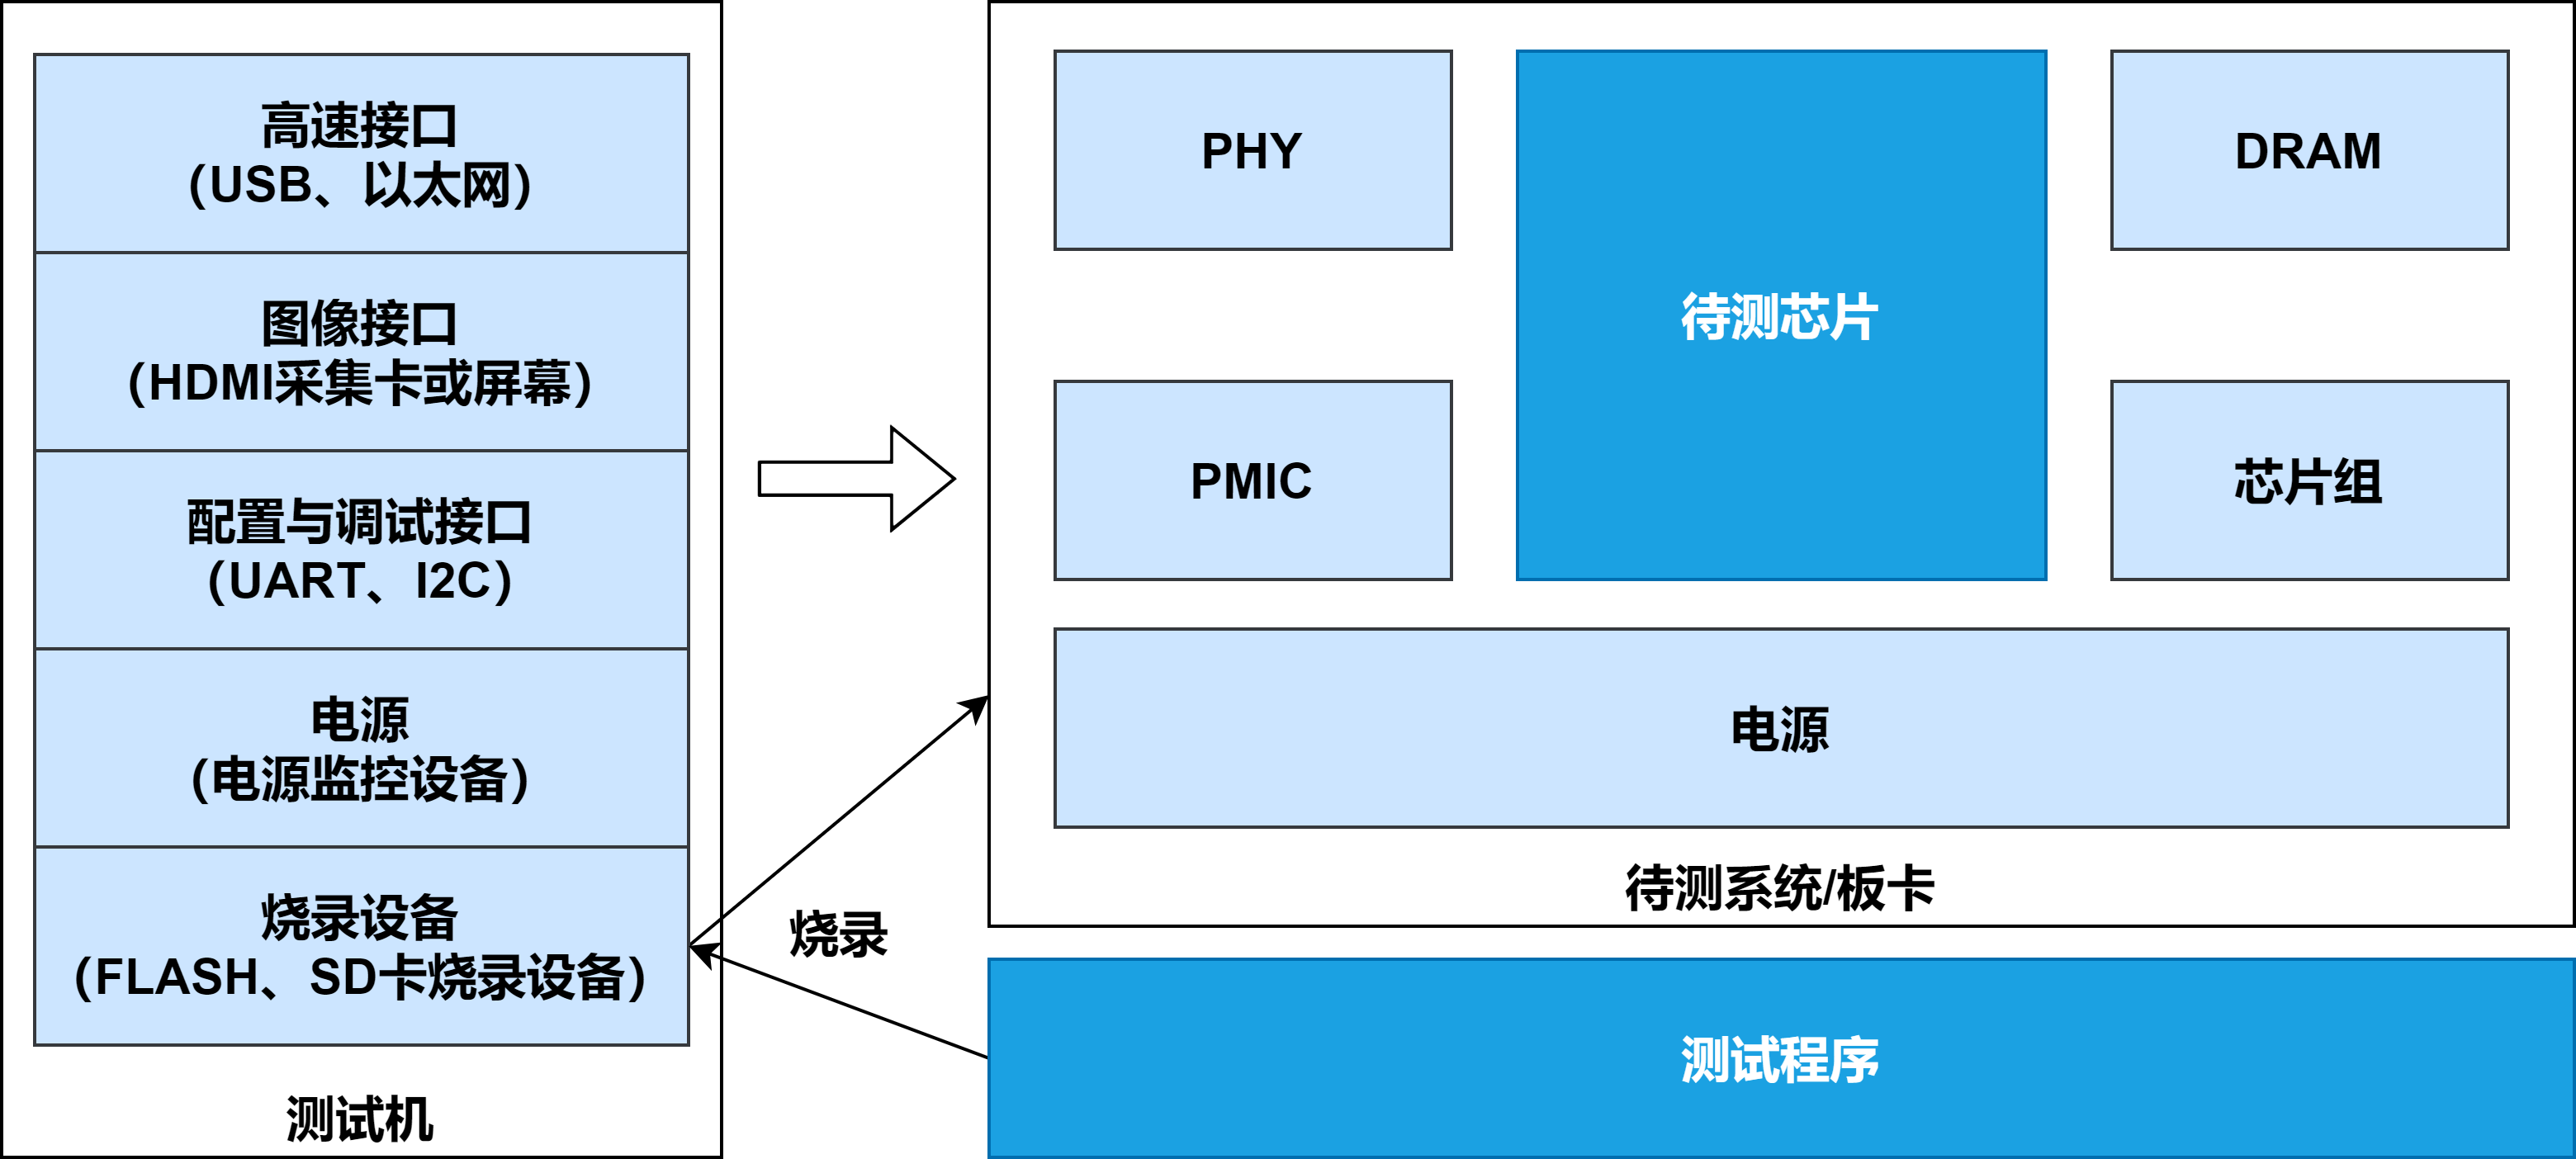
\includegraphics[width=1\linewidth]{assets/18/sys_level_test.png}
  \caption{SoC芯片测试系统}
  \label{fig:sys-level-test}
\end{figure}

\section{性能测试}\label{sec:18-test-and-show-006}

性能测试专注于评估芯片的速度、功耗和总体效率。在这个阶段，测试团队会通过一系列严格的测试来衡量芯片的性能指标，如处理速度、响应时间和功耗等。这些测试帮助识别可能的性能瓶颈和优化点。
性能测试对于确保芯片满足其市场和应用的要求至关重要，特别是对于高性能或低功耗应用的芯片。

对于处理器芯片，业内常使用 SPEC 套件对处理器进行测试。但需要注意的是，SPEC2006 套件及更新，需要至少 1G 的运行内存才可以正常工作，对于小于 1G 的设备，可以考虑使用 SPEC2000 或者其它嵌入式的性能测试工具。

对于嵌入式场景的处理器芯片，常用的测试工具包括 Coremark、Dhrystone 等。对其进行交叉编译，并在处理器芯片上运行即可。没有什么可以特别说明的。
